\subsection*{Reflected Cross-Site Scripting -- Search Parameter (XSS)}

\begin{table}[H]
\centering
\begin{tabular}{|l|p{10cm}|}
\hline
\textbf{Finding ID} & XSS \\
\hline
\textbf{Severity} & Medium \\
\hline
\textbf{CVSS 3.1 Score} & 6.1 (Medium) \\
\hline
\textbf{CVSS Vector} & \texttt{AV:N/AC:L/PR:N/UI:R/S:C/C:L/I:L/A:N} \\
\hline
\textbf{Status} & Confirmed \\
\hline
\textbf{OWASP Category} & A03:2021 -- Injection \\
\hline
\textbf{CWE} & CWE-79 -- Improper Neutralization of Input During Web Page Generation \\
\hline
\textbf{Affected Endpoint} & \texttt{GET /rest/products/search} \\
\hline
\textbf{Affected Parameter} & \texttt{q} \\
\hline
\end{tabular}
\caption{Reflected XSS finding details}
\end{table}

\subsubsection*{Description}

The product search feature was found to be vulnerable to
Reflected Cross-Site Scripting (XSS) through the \texttt{q}
parameter.

The application takes the value from the search parameter and
displays it back on the page without properly treating it as
plain text. Because of this, an attacker can create a specially
crafted search link containing JavaScript.

When a victim opens the malicious link, the injected JavaScript
can run in the victim's browser.

The malicious input is not stored in the application. It is
reflected back as part of the response, which is why this is
called \textbf{Reflected XSS}.

\subsubsection*{Methodology}

The normal product search request was first captured using
Burp Suite. The \texttt{q} parameter was then tested with
different XSS payloads using Burp Intruder.

The responses were checked to identify a payload that was
reflected by the application. The successful payload was then
opened in the browser. A JavaScript alert appeared, confirming
that the injected script was executed.

\subsubsection*{Steps to Reproduce}

\begin{enumerate}

    \item Open the OWASP Juice Shop product search feature.

    \item Capture the search request using Burp Suite.

    \item Send the request to Burp Intruder and select the
    \texttt{q} parameter as the injection point.

    \item Test the parameter with different XSS payloads.

    \item Check the responses to identify a payload that is
    reflected by the application.

    \item Open the successful payload in the browser.

    \item Observe the JavaScript alert displayed by the browser.
    This confirms that the injected script was executed.

\end{enumerate}

\subsubsection*{Evidence}

\begin{figure}[H]
    \centering
    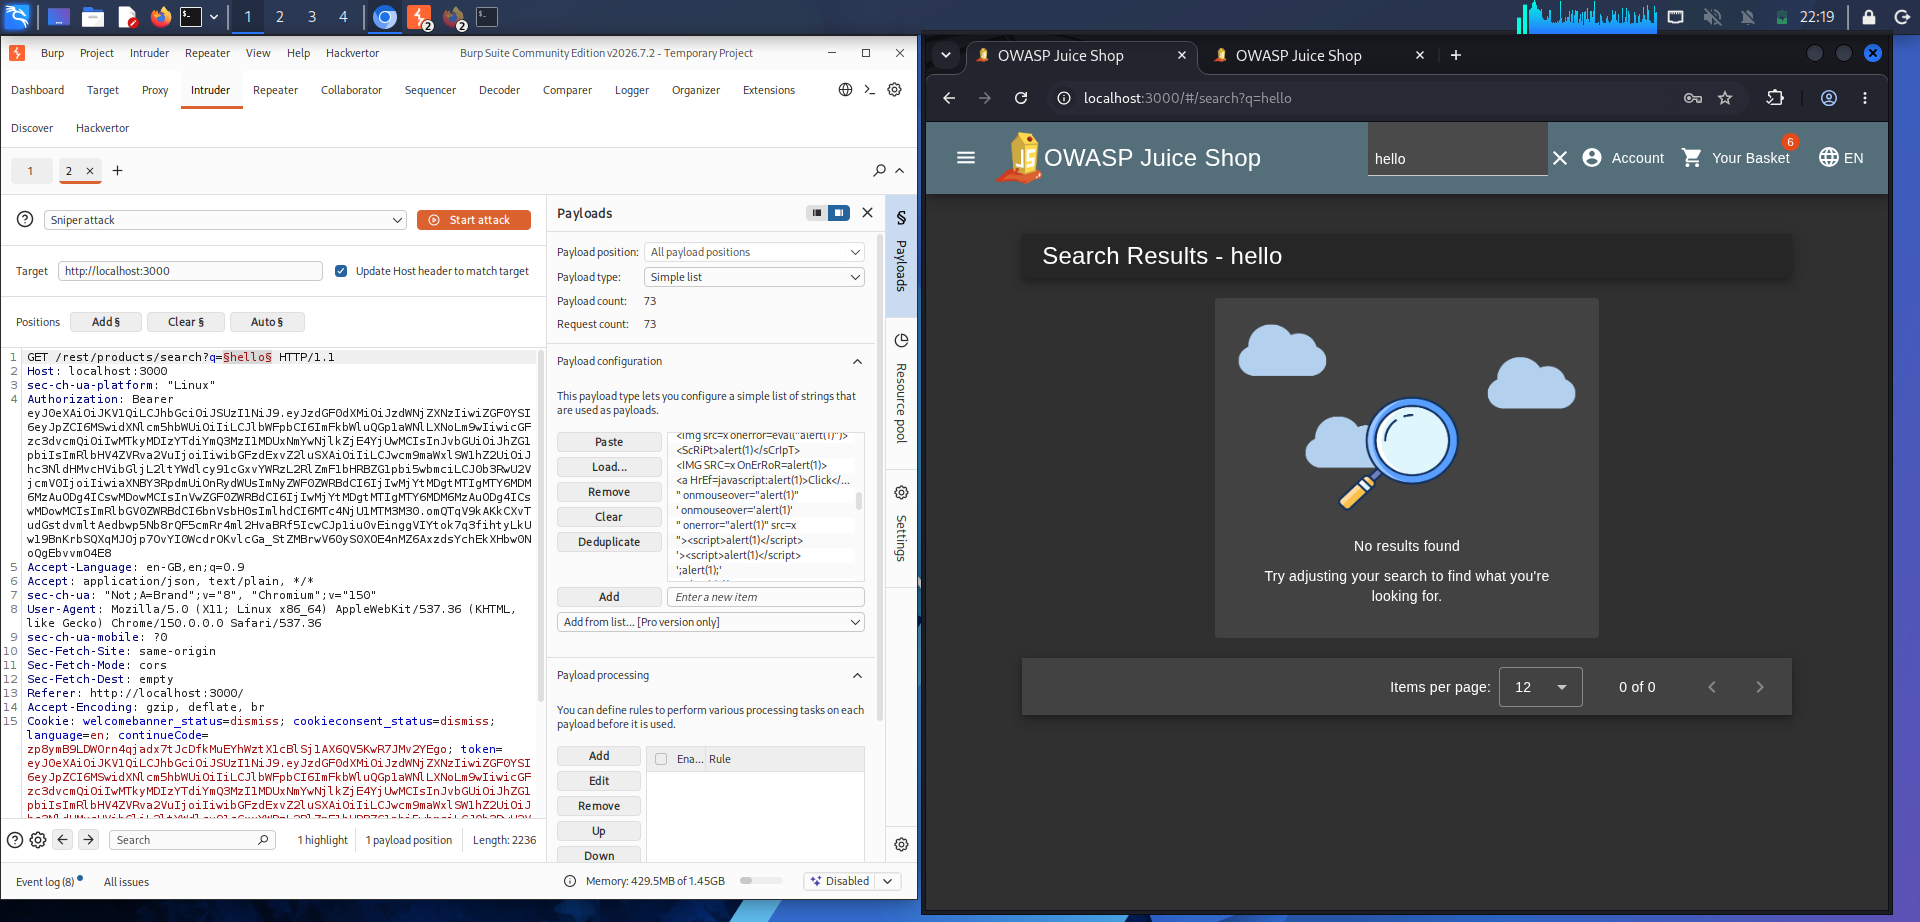
\includegraphics[width=0.9\textwidth]
    {evidence/phase4/xss-reflected/xss01-01-burp-intruder-payload-testing.png}
    \caption{Burp Intruder testing XSS payloads against the
    \texttt{q} parameter}
\end{figure}

\begin{figure}[H]
    \centering
    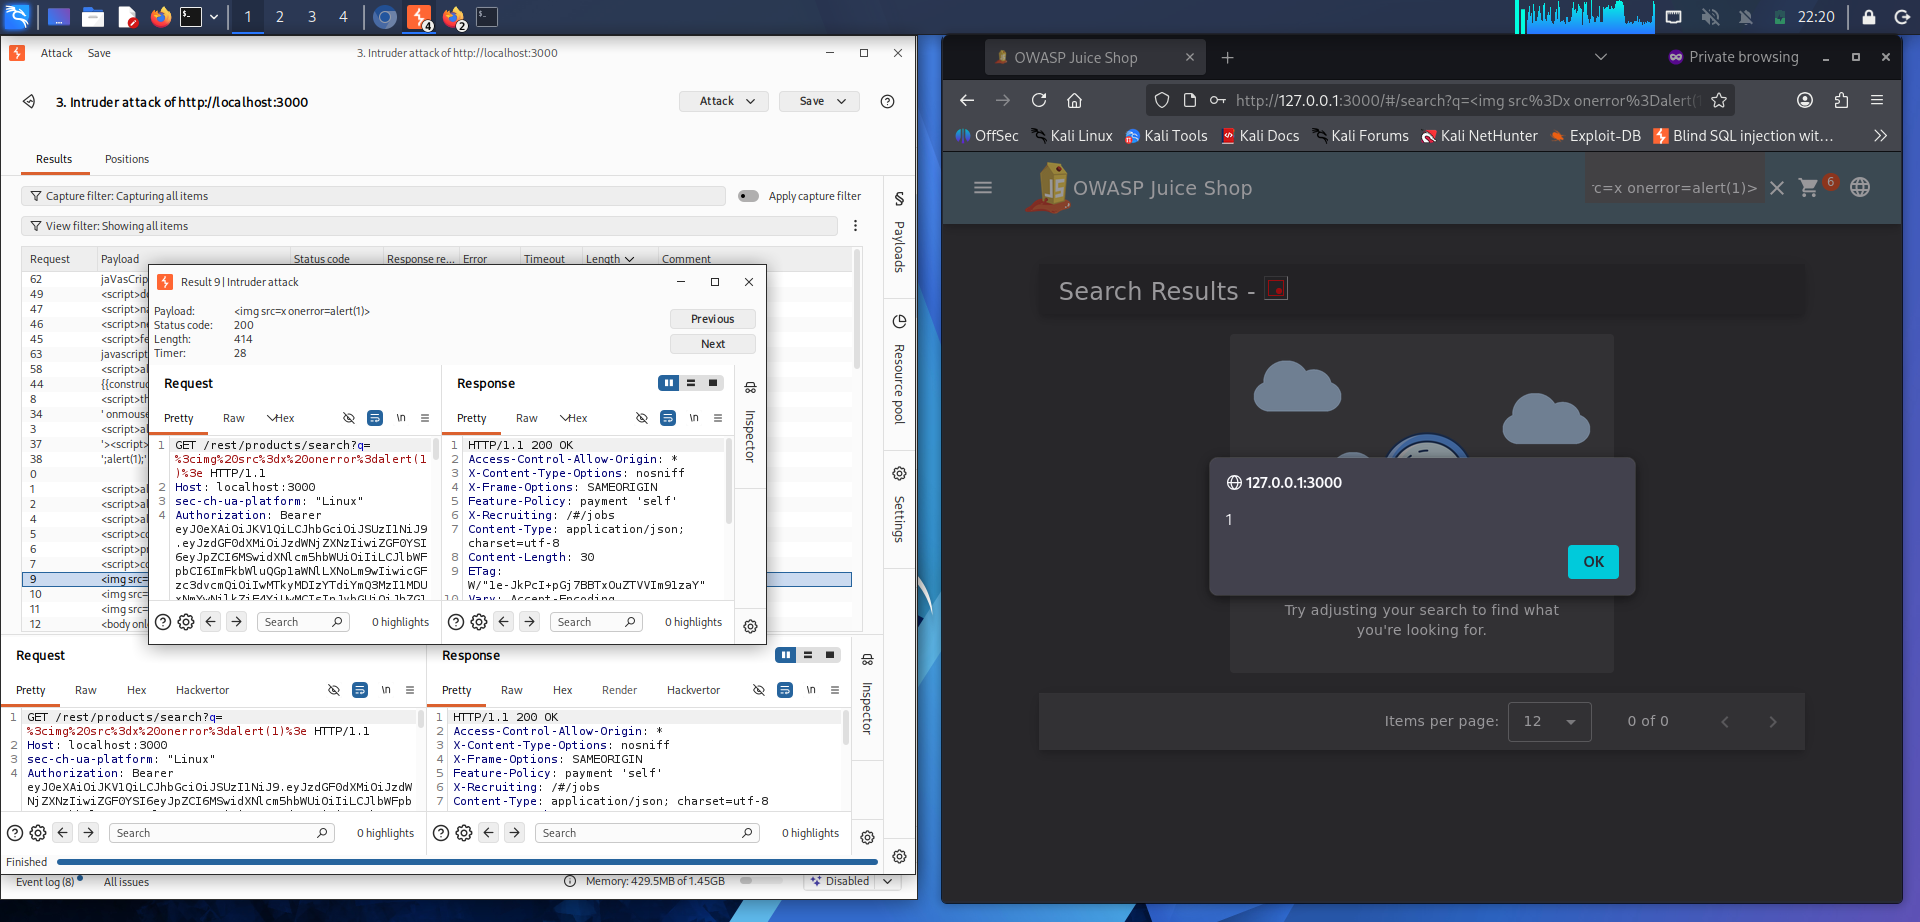
\includegraphics[width=0.9\textwidth]
    {evidence/phase4/xss-reflected/xss01-02-xss-payload-execution.png}
    \caption{JavaScript alert confirming execution of the
    injected XSS payload}
\end{figure}

\subsubsection*{Impact}

An attacker can create a malicious search link containing
JavaScript and send it to another user.

If the victim opens the link, the injected script can run in
the context of the OWASP Juice Shop application.

Depending on the user's privileges and the application's
security controls, this may allow the attacker to perform
actions using the victim's browser, modify displayed content,
redirect the victim to another page, or perform other
unauthorized actions.

\subsubsection*{Remediation}

\begin{itemize}

    \item Encode user-supplied input before displaying it on
    the webpage so that it is treated as text rather than
    executable JavaScript.

    \item Validate the \texttt{q} parameter on the server side
    and reject unexpected input where appropriate.

    \item Use secure output-encoding functions provided by the
    application's framework.

    \item Implement a strong Content Security Policy (CSP) as
    an additional layer of protection.

    \item Test all user-controlled input points for XSS before
    deploying the application.

\end{itemize}

\subsubsection*{Conclusion}

The Reflected XSS vulnerability in the product search parameter
was successfully confirmed through manual testing using Burp
Suite.

The injected payload was reflected by the application and
executed in the browser when the crafted input was opened.

The finding is therefore classified as a confirmed Medium-severity
Reflected Cross-Site Scripting vulnerability.